% Проверка векторных масок исполняемого кода на пустоту.
\subsection{Векторизация с проверкой векторных масок исполняемого кода на пустоту}\label{sec:text_4_vec_check_mask}

Рассмотрим небольшую модификацию слияния путей исполнения из раздела \ref{sec:text_4_vec_mrg_under_cond}, добавив проверку на пустоту векторых масок \texttt{COND} и \texttt{\textasciitilde COND}, под которыми исполняются векторизованные блоки \texttt{BLOCK A} и \texttt{BLOCK B} \cite{Rybakov2024VecComb} (см. рис.~\ref{fig:text_4_vec_check_mask_cond}). 

\begin{figure}[ht]
	\centering
	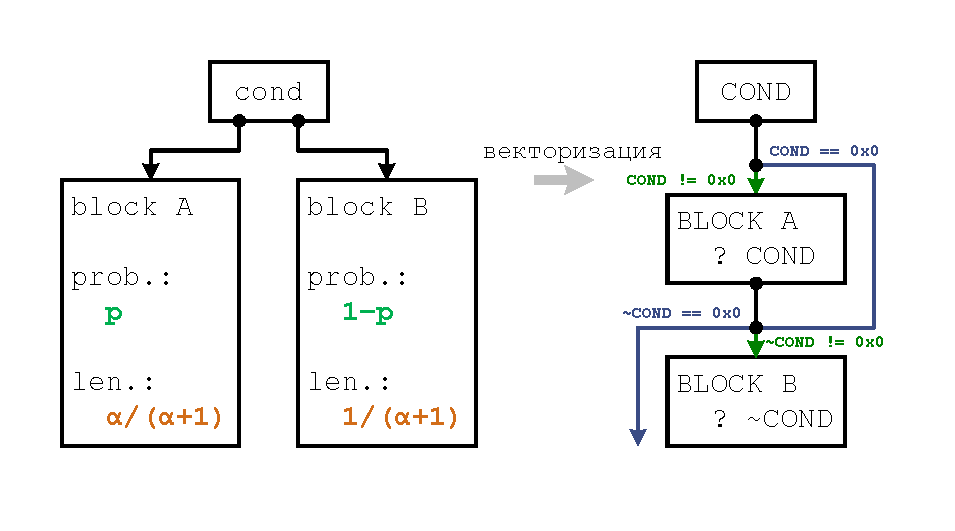
\includegraphics[width=0.8\textwidth]{./pics/text_4_vec_check_mask/cond.pdf}
	\caption{Схема векторизации участка программного кода, состоящего из одного условия и двух блоков, переход на которые осуществляется в соответствии с этим условием, с использованием проверок векторных масок на пустоту.}
	\label{fig:text_4_vec_check_mask_cond}
\end{figure}

Если векторная маска, под которой должен быть исполнен блок, пуста, то выполнять команды этого блока нет необходимости, поэтому проверка векторных масок на пустоту может повысить эффективность векторного кода.
Использование проверок векторных масок на пустоту оправдано, если вероятность появления пустых масок достаточно высока, а также исполняемый блок не является слишком коротким (в этом случае накладные расходы на лишнюю операцию сравнения и возможный переход нивелируют потенциальную пользу от применяемой оптимизации).
Скорректируем выражение для эффективности векторизации из \eqref{eqn:text_4_vec_mrg_under_cond_e} с учетом проверок векторных масок на пустоту.
Величина $T_1$ остается той же, что и в \eqref{eqn:text_4_vec_mrg_under_cond_t1}, а вот $T_w$ несколько изменится.
Если считать, что в каждом наборе обрабатываемых данных переход на тот или иной блок является случайной величиной, то вероятность пустой маски \texttt{COND} будет равна $(1 - p)^w$, тогда как вероятность пустой маски \texttt{\textasciitilde COND} равна $p^w$.
Тогда общая длина векторизованного кода может быть выражена как
\begin{equation}\label{eqn:text_4_vec_check_mask_tw}
	T_w = \left(1 - (1 - p)^w\right)\left(\frac{\alpha}{\alpha + 1}\right) + (1 - p^w)\left(\frac{1}{\alpha + 1}\right),
\end{equation}

а эффективность векторизации примет следующий вид:
\begin{equation}\label{eqn:text_4_vec_check_mask_e}
	e = \frac{ p(\alpha - 1) + 1 }{\left(1 - (1 - p)^w\right) \alpha + (1 - p^w) }.
\end{equation}

На рис.~\ref{fig:text_4_vec_check_mask_chart_e_merged} представлены зависимости эффективности векторизации \eqref{eqn:text_4_vec_check_mask_e} при разных значениям параметра $\alpha$ с учетом проверок масок на пустоту для ширины векторизации $w = 16$, что соответствует использованию вещественного формата данных одинарной точности в 512-битных регистрах.

\begin{figure}[ht]
	\centering
		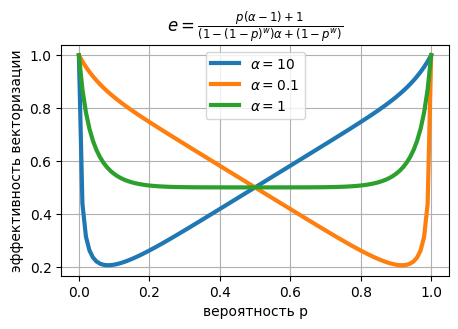
\includegraphics[width=0.6\textwidth]{./pics/text_4_vec_check_mask/chart_e_merged.png}
	\caption{Графики зависимостей эффективности векторизации от вероятности перехода на \texttt{block A} при значениях отношения длин блоков \texttt{block A} и \texttt{block B} $\alpha = 10,0$, $\alpha = 0,1$ и $\alpha = 1,0$ и при использовании слияния путей исполнения с проверкой масок на пустоту.}
	\label{fig:text_4_vec_check_mask_chart_e_merged}
\end{figure}

Из рис.~\ref{fig:text_4_vec_check_mask_chart_e_merged} видно, что эффективность векторизации возрастает, если значение вероятности перехода на один из блоков близко к единице, однако в среднем вероятность векторизации остается невысокой.
